\section{Evaluation}\label{sec:experiment}

In this section, we evaluate our proof-of-concept system 
for speculative nondeterminism by using benchmarks based on
the three examples described in Section \ref{sec:examples}.
In fact, the examples are very similar to the actual benchmarks run.

\begin{description}
\item[Flight Reservation (FR)]
We use the same strategy described in Listing \ref{lst:tsell}
and \ref{lst:tbuy}, but on a larger airline map
\footnote{We use the HA30 dataset which is available 
at \url{http://people.sc.fsu.edu/~jburkardt/datasets/cities/cities.html}.}
of 30 international cities. 
\item[Stock Trading (ST)]
We use the same strategy described in Listing \ref{lst:trader},
but limit the number of trades to be exactly 3. 
The total number of stocks is 10 and the initial available shares
are proportional to the number of traders. 
For each stock, we replay 1000 data points which are real stock market
data in the U.S.
\item[Dining Philosophers (DP)]
This example in the benchmark is exactly the same as shown in 
Listing \ref{lst:dpinit} and \ref{lst:dp}.
\end{description}

We evaluate our runtime system running these benchmarks
on Linux (2.6.18) with Intel Xeon E5520 2.2GHz CPU and 24GB RAM.
Both the prototype system and benchmark programs are written in Erlang,
and run in Erlang VM (64-bit R15B02) with HiPE and SMP (4 schedulers, i.e. 4 cores are used) enabled.

\begin{figure*}[tb]
\centering
% FR
\subfigure[FR: Max Memory Consumption]{
  \label{fig:fr-mem}
  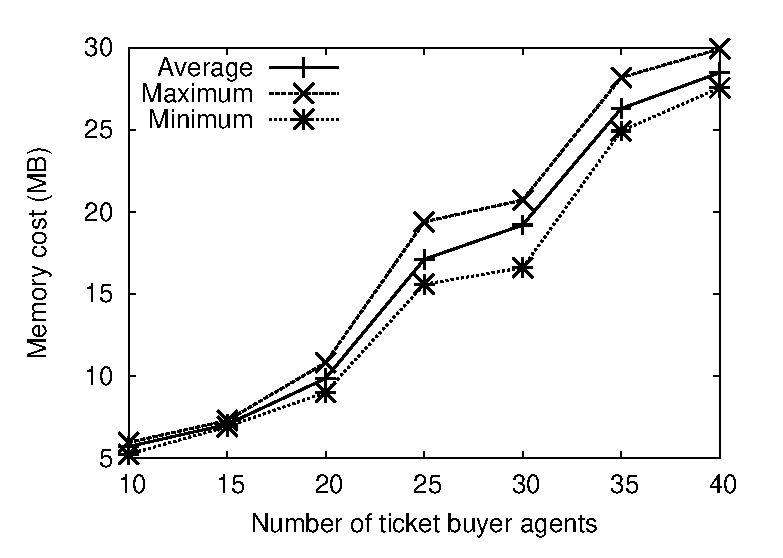
\epsfig{file=eps/fr-mem.eps,width=0.24\textwidth}}
\subfigure[FR: Max \# of Concur. Worlds]{
  \label{fig:fr-world}
  \epsfig{file=eps/fr-world.eps,width=0.24\textwidth}}
\subfigure[FR: Total CPU Time]{
  \label{fig:fr-cpu}
  \epsfig{file=eps/fr-cpu.eps,width=0.24\textwidth}}
\subfigure[FR: \% Time Saving Due to Exit]{
  \label{fig:fr-exit}
  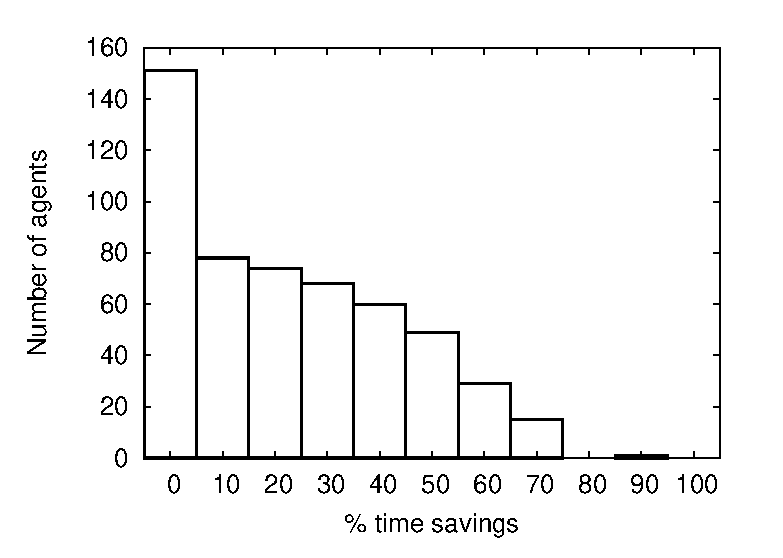
\epsfig{file=eps/fr-exit.eps,width=0.24\textwidth}}
% ST
\subfigure[ST: Max Memory Consumption]{
  \label{fig:st-mem}
  \epsfig{file=eps/st-mem.eps,width=0.24\textwidth}}
\subfigure[ST: Max \# of Concur. Worlds]{
  \label{fig:st-world}
  \epsfig{file=eps/st-world.eps,width=0.24\textwidth}}
\subfigure[ST: Total CPU Time]{
  \label{fig:st-cpu}
  \epsfig{file=eps/st-cpu.eps,width=0.24\textwidth}}
\subfigure[ST: \% Time Saving Due to Exit]{
  \label{fig:st-exit}
  \epsfig{file=eps/st-exit.eps,width=0.24\textwidth}}
% DP
\subfigure[DP: Max Memory Consumption]{
  \label{fig:dp-mem}
  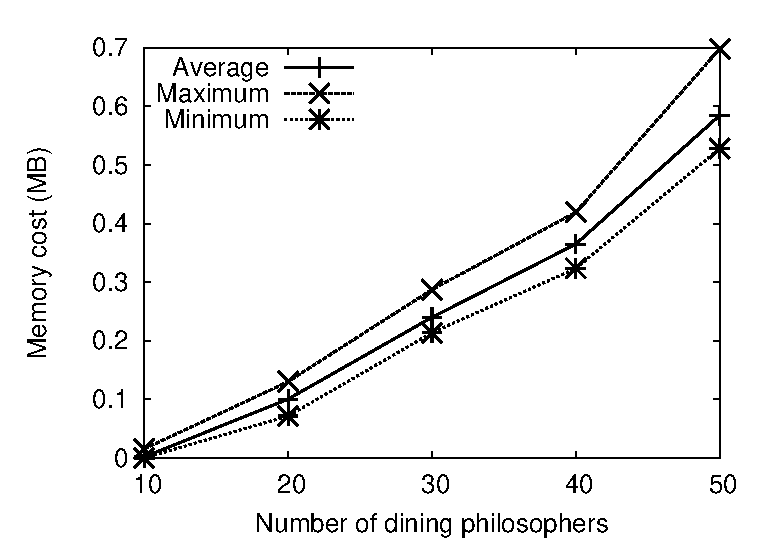
\epsfig{file=eps/dp-mem.eps,width=0.24\textwidth}}
\subfigure[DP: Max \# of Concur. Worlds]{
  \label{fig:dp-world}
  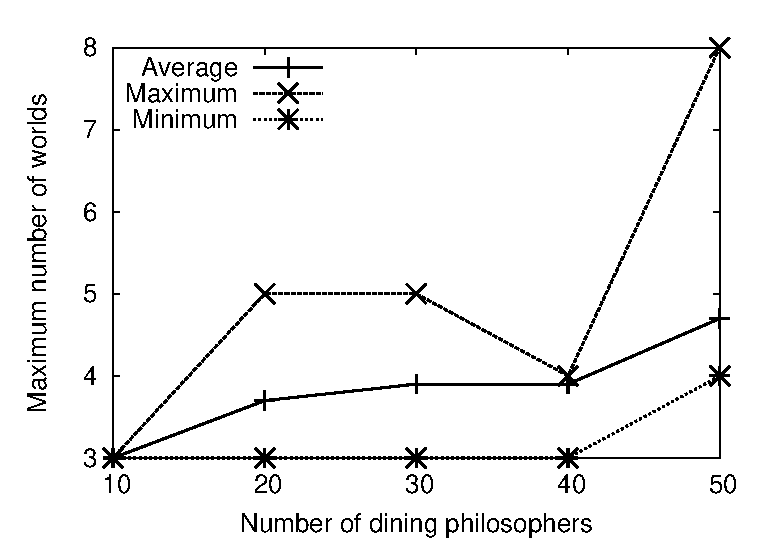
\epsfig{file=eps/dp-world.eps,width=0.24\textwidth}}
\subfigure[DP: Total CPU Time]{
  \label{fig:dp-cpu}
  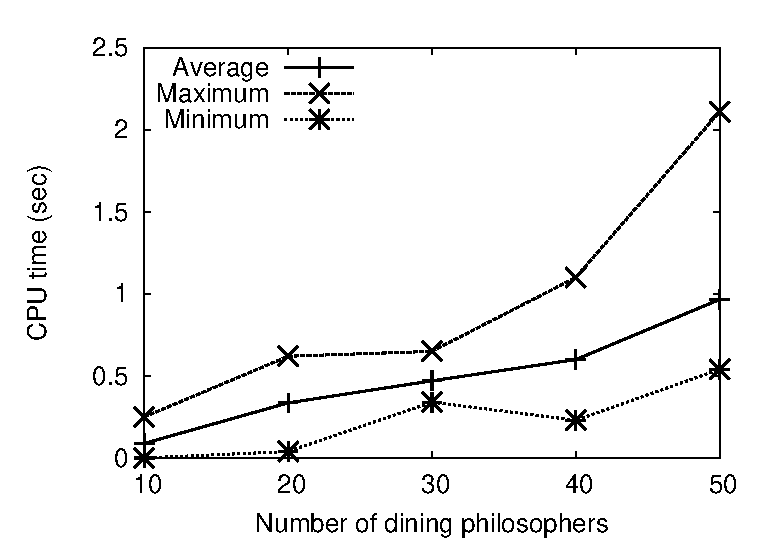
\epsfig{file=eps/dp-cpu.eps,width=0.24\textwidth}}
\subfigure[DP: \% Time Saving Due to Exit]{
  \label{fig:dp-exit}
  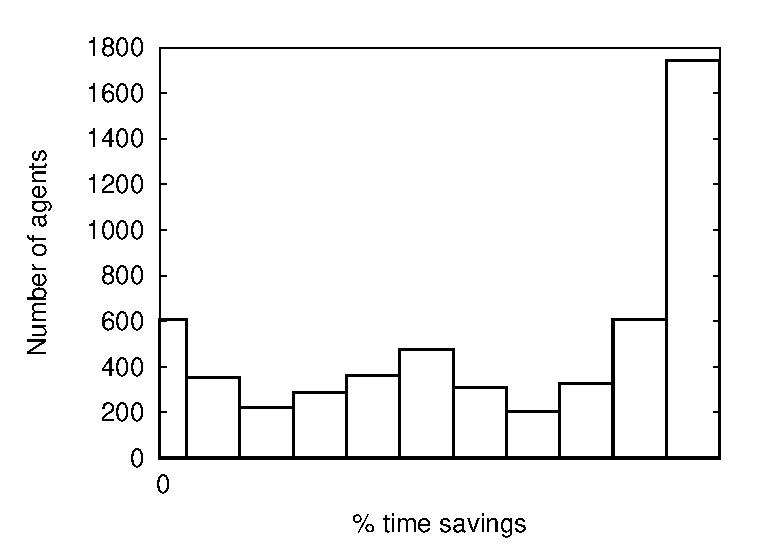
\epsfig{file=eps/dp-exit.eps,width=0.24\textwidth}}
%
\caption{Evaluation Results}
\label{fig:eval}
\end{figure*}

In each benchmark, we conducted several experiments with different number of 
concurrent agents. We ran each experiment 10 times and record the average,
maximum and minimum values for three key metrics: 
maximum memory consumption, maximum number of simultaneous worlds and 
total CPU time. 
In addition, we record the percentage time savings of each agent by
\begin{equation*}
\frac{\rm{exit\ time\ of\ last\ agent\ in\ system} - 
\rm{exit\ time\ of\ this\ agent}}
{\rm{exit\ time\ of\ last\ agent\ in\ system}}
\end{equation*}
because without exit mechanism in the system, all agents would have waited
till the last agent completes to exit from the system together. 

Figure \ref{fig:eval} shows the results.
We can see that even though theoretically the
maximum number of worlds in these examples are prohibitively large 
(i.e., $2^n$),
in reality, with the help of the commit operators, we can keep
the size of the universe as well as other computation costs
down to very manageable. In other words, given well programmed agents and a
reasonable commit mechanism, the prototype system can manage 
the exponentiality inherent in the problems while achieving 
solutions for all agents in reasonable time. 
However, as a proof-of-concept prototype, the system can also 
be affected by some special combination of choices and realtime events. 
For example, in Figure \ref{fig:st-mem} and \ref{fig:st-world} 
of the ST benchmark, the anomalies can be caused by a special combination 
of trading strategies which leads to resource contention. 
Different number of agents also slightly affects the scheduling so 
some realtime price updates can be missed by the agents.
Furthermore, as our implementation is in pure Erlang, there is no shared
state, and message passing is the only way which agents interact with the
system. While this has more overhead, it allows the system to be potentially
distributed.

Furthermore, Figure \ref{fig:fr-exit}, \ref{fig:st-exit} and 
\ref{fig:dp-exit} show the distributions of agents on the time savings due to
the exit semantics. Most of the agents save at least half of the overall time
with the exit semantics implemented. FR has slightly less savings in time because
most of the worlds only have limited resources for the agents to commit. 
Overall, the results clearly demonstrate
that the exit mechanism significantly improves the user responsiveness and 
the efficiency of the computation. A carefully engineered
application which uses the speculative nondeterminism model
should be even more efficient.
